\chapter{Planification}

\section{Hiérarchie des tâches}

\begin{figure}[H]
	\centering
	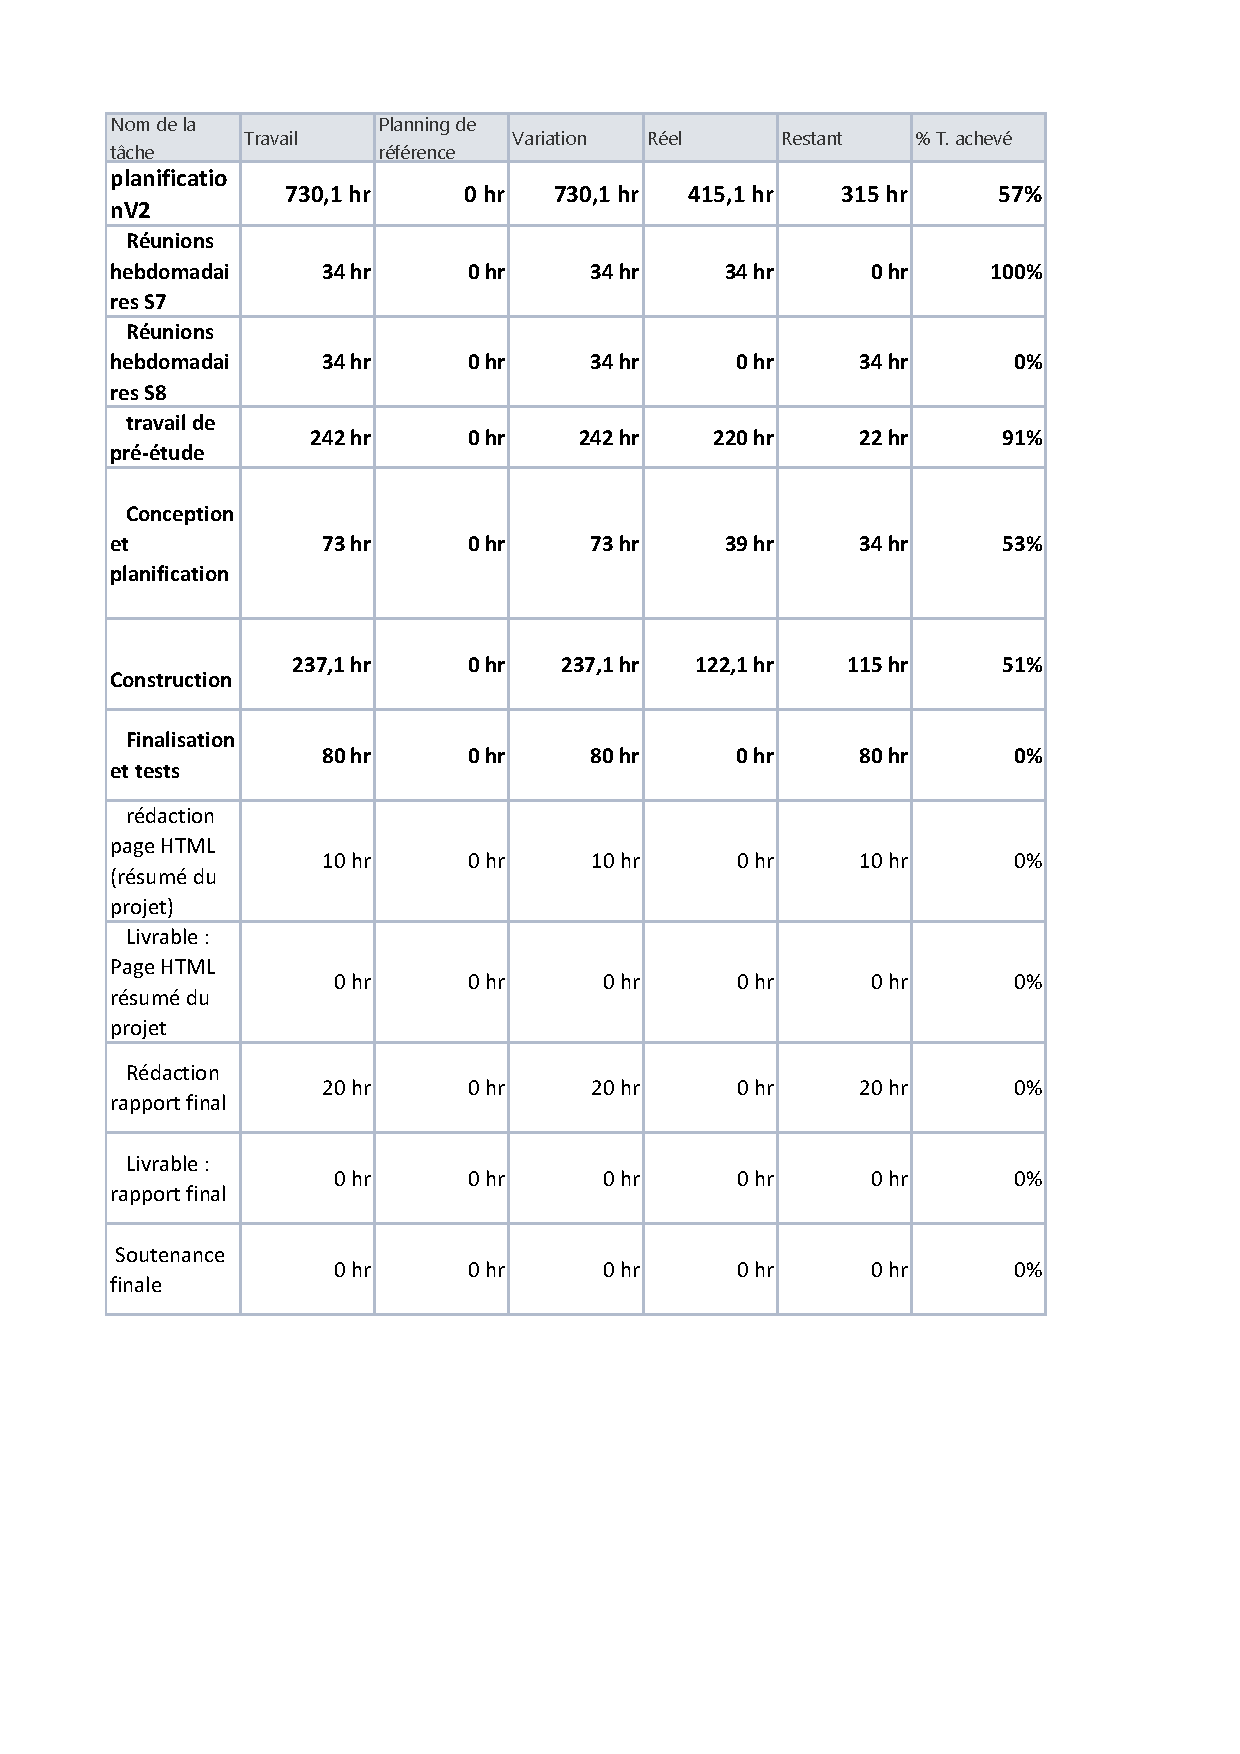
\includegraphics[scale=0.7]{images/taches.pdf}
	\caption{Tableau des tâches}
\end{figure}

\section{Affectation des ressources}
TO ADD : TABLEAU D'OCCUPATION DES RESSOURCES


\section{Planning}
\begin{figure}[H]
	\centering
	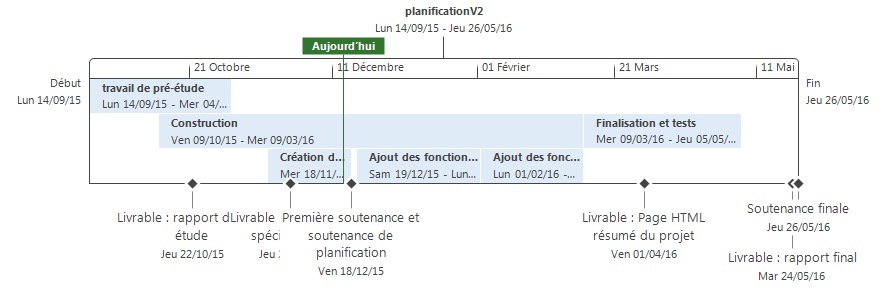
\includegraphics[scale=0.7]{images/chrono_planif.png}
	\caption{Chronologie du projet}
\end{figure}

Notre planning restera étroitement lié aux différentes étapes du suivi des mobilités. La construction de l'application se fera donc en trois étapes :
\begin{itemize}
 \item la création d'un prototype proposant les fonctionnalités nécessaires à la première étape (vœux et affectations).
 \item la gestion des fichiers nécessaires à la mobilité (dépôt sur le site, et apposition électronique de la signature).
 \item le suivi des étudiants à l'étranger.
\end{itemize}
Nous travailleront donc de façon itérative, en proposant une application fonctionnelle, un peu plus complète à la fin de chaque étape.


Suite à cela, nous avons réservé beaucoup de temps à la finalisation du projet. Celui-ci étant destiné à devenir une application pérenne, au service de l'INSA de Rennes, il est nécessaire de s'assurer de sa stabilité. Nous travailleront aussi le design du site durant cette étape. 

\begin{figure}[H]
	\centering
	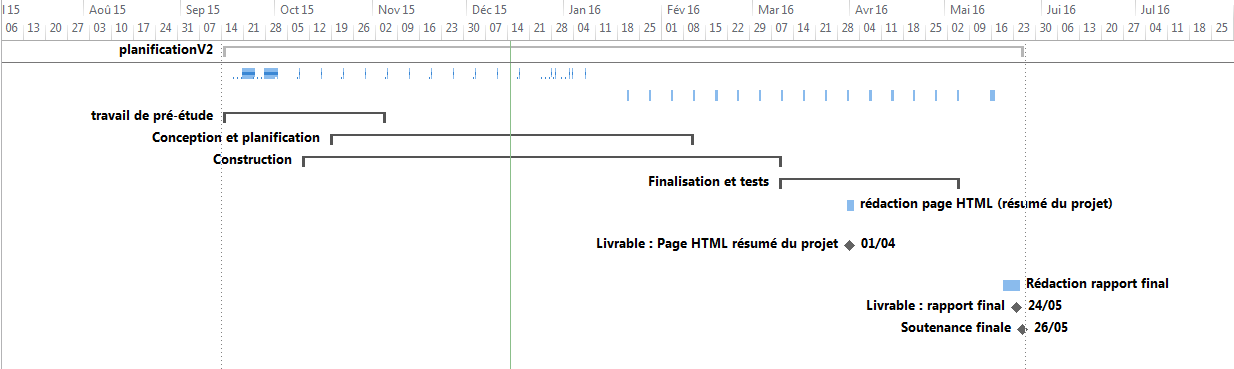
\includegraphics[scale=0.5]{images/gant.PNG}
	\caption{GANT (réduit aux grandes parties du projet)}
\end{figure}

